%\documentstyle[epsf,twocolumn]{jarticle}       %LaTeX2e仕様
\documentclass[twocolumn]{jarticle}     %pLaTeX2e仕様(platex.exeの場合)
%\documentclass[twocolumn]{ujarticle}     %pLaTeX2e仕様(uplatex.exeの場合)
%%%%%%%%%%%%%%%%%%%%%%%%%%%%%%%%%%%%%%%%%%%%%%%%%%%%%%%%%%%%%%
%%
%%  基本バージョン
%%
%%%%%%%%%%%%%%%%%%%%%%%%%%%%%%%%%%%%%%%%%%%%%%%%%%%%%%%%%%%%%%%%
\setlength{\topmargin}{-45pt}
%\setlength{\oddsidemargin}{0cm} 
\setlength{\oddsidemargin}{-7.5mm}
%\setlength{\evensidemargin}{0cm} 
\setlength{\textheight}{24.1cm}
%setlength{\textheight}{25cm} 
\setlength{\textwidth}{17.4cm}
%\setlength{\textwidth}{172mm} 
\setlength{\columnsep}{11mm}

\kanjiskip=.07zw plus.5pt minus.5pt


% 【節が変わるごとに (1.1)(1.2) … (2.1)(2.2) と数式番号をつけるとき】
%\makeatletter
%\renewcommand{\theequation}{%
%\thesection.\arabic{equation}} %\@addtoreset{equation}{section}
%\makeatother

%\renewcommand{\arraystretch}{0.95} 行間の設定

%%%%%%%%%%%%%%%%%%%%%%%%%%%%%%%%%%%%%%%%%%%%%%%%%%%%%%%%
\usepackage[dvipdfmx]{graphicx}   %pLaTeX2e仕様(\documentstyle ->\documentclass)\documentclass[dvipdfmx]{graphicx}
\usepackage[dvipdfmx]{color}
\usepackage[subrefformat=parens]{subcaption}
\usepackage{colortbl}
\usepackage{multicol}
%%%%%%%%%%%%%%%%%%%%%%%%%%%%%%%%%%%%%%%%%%%%%%%%%%%%%%%%

\begin{document}

\twocolumn[
\noindent

\hspace{1em}
\today
\hfill
\ \ 細川 岳大

\vspace{2mm}

\hrule

\begin{center}
{\Large \bf 進捗報告}
\end{center}
\hrule
\vspace{3mm}
]

% ‚ここから 文章 Start!

\section{今週やったこと}

Virtual Adversarial Training(:VAT)の実験をしたが,うまくいかなかった.\\
前回batchが乗らないといっていたが乗るように修正した.
しかし,やはりaccuracyが上がらなかったので,VAT中のkldを除いた純粋なCNNで
動かしてみるとそこについては問題がなかったためkldのlossの伝播がうまくいっていないと思われる.\\
\\
とりあえず他にあったkerasの実装で試してみることにした.
データセットはmnistでラベル付き100枚,ラベルなし59900枚,validationを10000枚で実験を行った.
modelはフィルタ数32,64,128にdense層2枚のCNN,accuracyは最終的に95\%で元論文では98.7\%
まででており,ある程度の精度が出ていると思われる.また,同model1で100枚のラベル付きのみでは78\%程度のため
うまくいっているといえる.\\
しかし,この実装で回したとき,1epochに5分かかってしまっているので,
GAをより多く回すためにはpytorchでのかかる時間も見てあげる必要があると思われる.

\begin{figure}[hp]
	\centering
	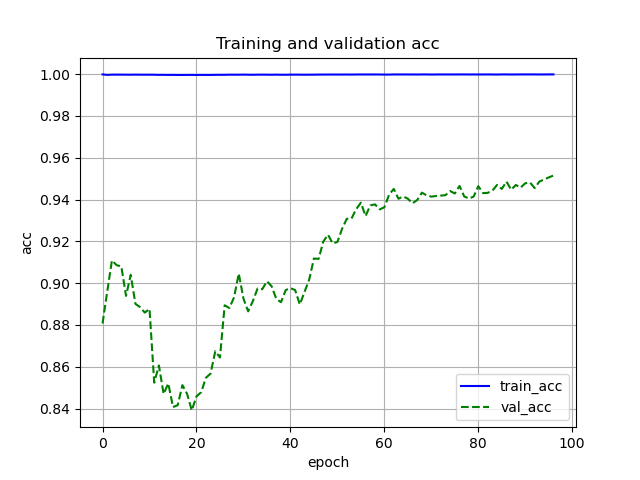
\includegraphics[scale=0.7]{acc__.png}
	\caption{accの推移\label{fig:graph}}
\end{figure}


\section{来週の課題}
\begin{itemize}
	\item pytorchのソースコードを見直し,実験を行う
\end{itemize}

\end{document}


